\chapter{Proposed methods}
\label{cha:methodology}

This chapter introduces the theoretical framework that forms the core of this work, focused on the use of the attentions within LDMs for explainability purposes and their alignment with different objects in synthetically produced urban scenes.

Initially, in Section \ref{cha:methodology-daam}, we present the theory behind the DAAM explainability method \cite{DAAM}. This method allows the creation of attribution maps that relate the input text to the images generated by an LDM, further enabling the generation of segmentation masks. By attributing the influence of input tokens in the generated images, DAAM provides a valuable tool for understanding the connection between textual prompts and visual output.

Proceeding further, in Section \ref{cha:methodology-ov-daam}, we propose an extension of this explainability method, referred to as Open Vocabulary DAAM. This extension overcomes the limitation of the original DAAM by enabling the construction of attribution maps for any given text, not restricted to the tokens used during image generation. Open Vocabulary DAAM enhances the flexibility and applicability of the method, allowing for the exploration of diverse textual prompts and their influence on the generated images.

Finally, in Section \ref{cha:methodology-ov-daam-optimization}, we propose a methodology for optimizing an input text embedding to maximize the Intersection over Union (IoU) of DAAM-generated masks. This optimization process aims to align the generated masks more closely with the desired semantic segmentation masks, enhancing the fidelity and accuracy of synthetically generated ground truth.

Through this examination, we aim to cover the DAAM theoretical framework, its potential pitfalls, and paths for advancement. This foundation sets the stage for the empirical explorations presented in Chapter \ref{cha:experiments}, where we evaluate and analyze the practical implications of these methods on the task of semantic segmentation in urban scenes.

\section{Diffusion Attentive Attribution Maps}
\label{cha:methodology-daam}


The Diffusion Attentive Attribution Maps (DAAM) method represents a pioneering work in enhancing the explainability of text-to-image diffusion models \cite{DAAM}. This technique facilitates the attribution of individual input words' influence on the synthetic images generated by the model.

By leveraging the attention mechanisms activated during the diffusion process, 
DAAM constructs heatmaps corresponding to each token used as input.
These attention-based heatmaps align with semantically significant image areas, capturing not only primary objects but also abstract concepts embedded within the image, such as adjectives, verbs, or semantic relationships between words \cite{DAAM}.

For example, Figure \ref{fig:daam-example} presents an image generated with Stable Diffusion \cite{rombach2022high} using the text prompt ``A car in an urban environment'' (Figure \ref{fig:daam-example-image}), accompanied by DAAMs for each token in the prompt.  This prompt was chosen for this example after practical tests with various prompts, where it generated examples with a main object in the image within urban scenes, which aligns with the research context of this work. Each heatmap corresponds to a specific word in the input text, including the starting and ending special tokens, providing insights into how each word influences different regions of the generated image.
The following observations can be made from the heatmaps:


\begin{itemize}
\item \textlangle SOT\textrangle\ (\ref{fig:daam-example-image-1}): The heatmap primarily accumulates information from the image background, such as the city street and building. This attention pattern is common for the onset token, which tends to gather attention from regions not influenced by other tokens \cite{DAAM}.
\item ``a'' (\ref{fig:daam-example-image-2}): The heatmap exhibits a dispersed pattern across the entire image, suggesting that the word ``a'' influences various regions without a specific focus.
\item ``car'' (\ref{fig:daam-example-image-3}): The heatmap precisely outlines the shape of the car in the center of the image, highlighting the strong influence of the word ``car'' on that object.
\item ``in'' (\ref{fig:daam-example-image-4}): The heatmap focuses on the region of the car, indicating an semantic association between the word ``in'' and ``car''.
\item ``an'' (\ref{fig:daam-example-image-5}): The heatmap centers on the shape of the car but contains more noise, suggesting some ambiguity or uncertainty in the attribution.
\item ``urban'' (\ref{fig:daam-example-image-6}) and ``environment'' (\ref{fig:daam-example-image-7}): The heatmaps draw attention from various regions of the image, particularly the background building, indicating a strong association between these words and the elements of the environment.
\item \textlangle EOT\textrangle\ (\ref{fig:daam-example-image-8}): The heatmap complements the onset token's heatmap (\textlangle SOT\textrangle), with a specific focus on the car's location during the image generation process.
\end{itemize}


\begin{figure}
\centering
  % First column
  \begin{subfigure}{0.32\columnwidth}
   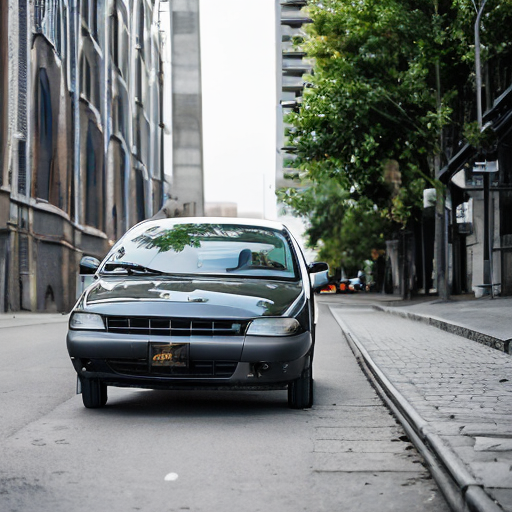
\includegraphics[width=\columnwidth]{img/3-methodology/example_daam.png}
   \caption{Image generated}
   \label{fig:daam-example-image}
  \end{subfigure}
  \begin{subfigure}{0.32\columnwidth}
   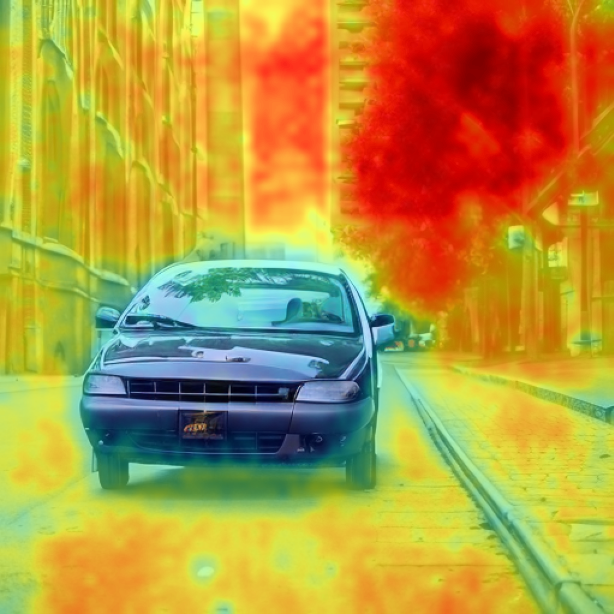
\includegraphics[width=\columnwidth]{img/3-methodology/example_daam_heatmap_SoT.png}
   \caption{\textlangle SOT\textrangle}
   \label{fig:daam-example-image-1}
  \end{subfigure}
  \begin{subfigure}{0.32\columnwidth}
   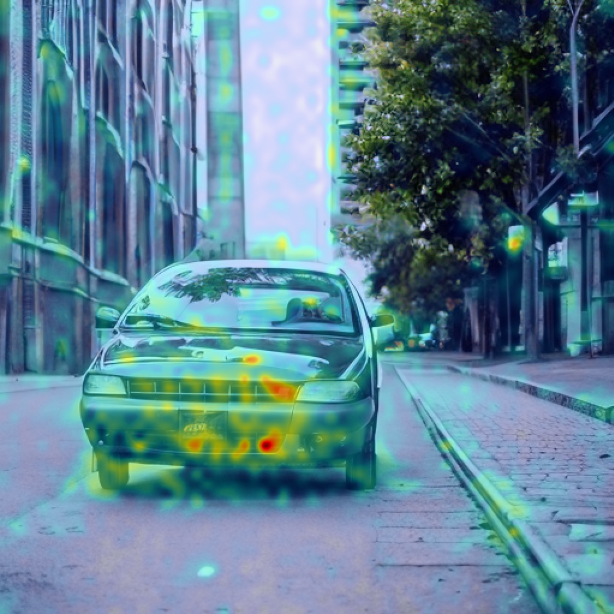
\includegraphics[width=\columnwidth]{img/3-methodology/example_daam_heatmap_a.png}
   \caption{``a''}
   \label{fig:daam-example-image-2}
  \end{subfigure}
  \par\bigskip
  % Second column
  \begin{subfigure}{0.32\columnwidth}
   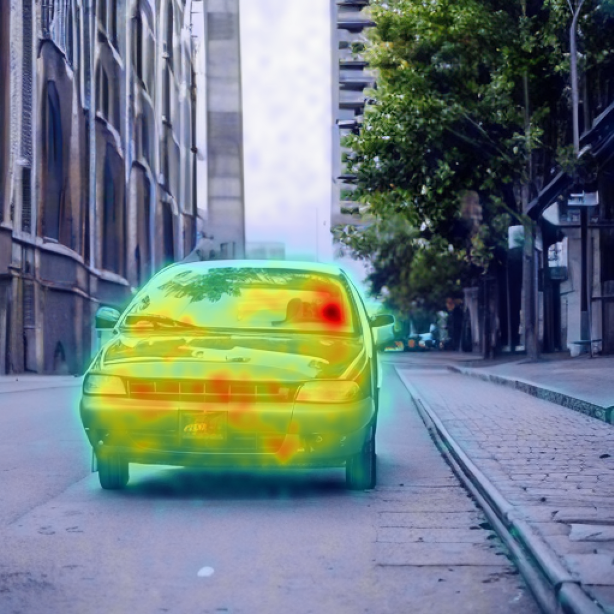
\includegraphics[width=\columnwidth]{img/3-methodology/example_daam_heatmap_car.png}
   \caption{``car''}
   \label{fig:daam-example-image-3}
  \end{subfigure}
  \begin{subfigure}{0.32\columnwidth}
   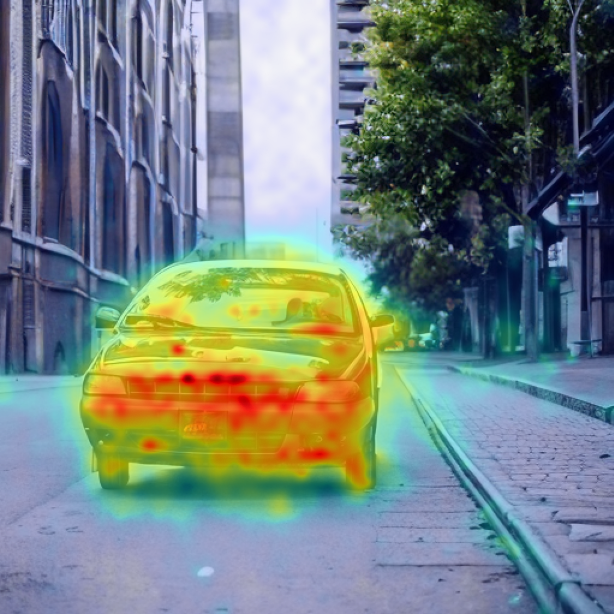
\includegraphics[width=\columnwidth]{img/3-methodology/example_daam_heatmap_in.png}
   \caption{``in''}
   \label{fig:daam-example-image-4}
  \end{subfigure}
  \begin{subfigure}{0.32\columnwidth}
   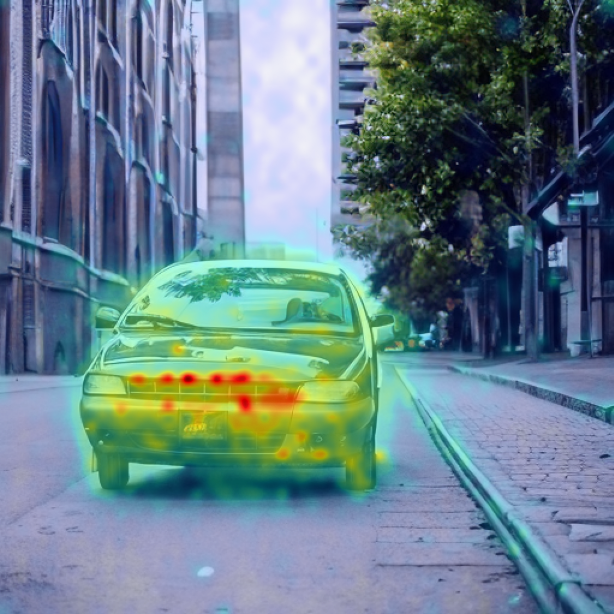
\includegraphics[width=\columnwidth]{img/3-methodology/example_daam_heatmap_an.png}
   \caption{``an''}
   \label{fig:daam-example-image-5}
  \end{subfigure}
  \par\bigskip
    % Third column
  \begin{subfigure}{0.32\columnwidth}
   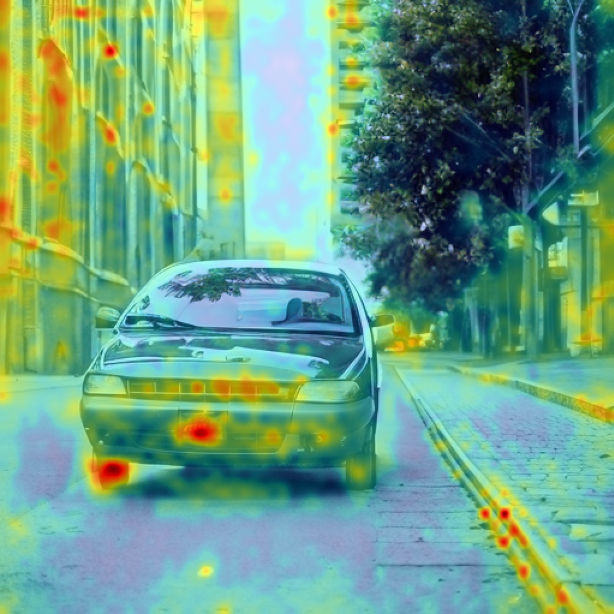
\includegraphics[width=\columnwidth]{img/3-methodology/example_daam_heatmap_urban.png}
   \caption{``urban''}
   \label{fig:daam-example-image-6}
  \end{subfigure}
  \begin{subfigure}{0.32\columnwidth}
   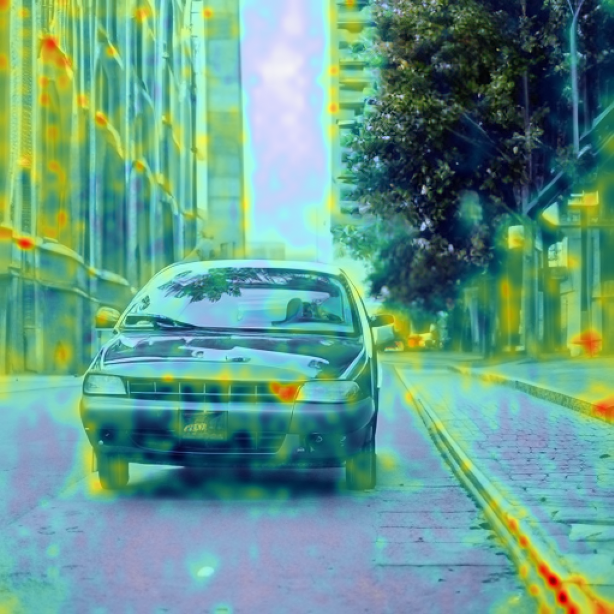
\includegraphics[width=\columnwidth]{img/3-methodology/example_daam_heatmap_environment.png}
   \caption{``environment''}
   \label{fig:daam-example-image-7}
  \end{subfigure}
  \begin{subfigure}{0.32\columnwidth}
   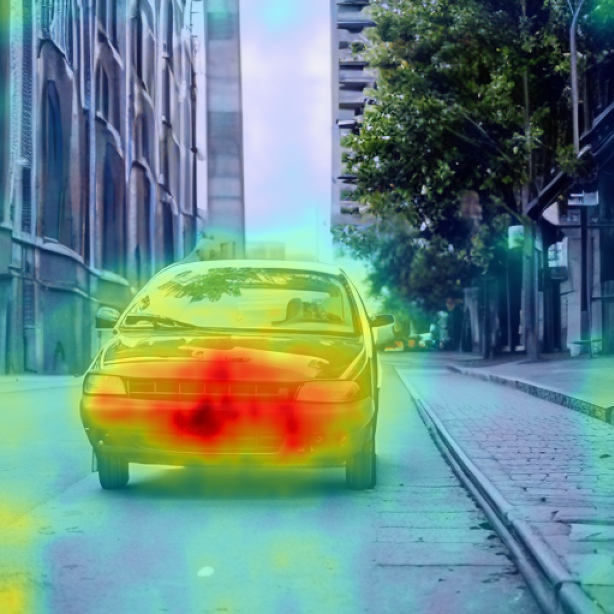
\includegraphics[width=\columnwidth]{img/3-methodology/example_daam_heatmap_EoT.png}
   \caption{\textlangle EOT\textrangle}
   \label{fig:daam-example-image-8}
   \end{subfigure}
  \caption[Example of Diffusion Attentive Attribution Maps]{An image generated using Stable Diffusion with the text ``A car in an urban environment'' along with overlayed DAAMs for each token.}
  \label{fig:daam-example}
  \end{figure}



This example illustrates the information provided by DAAM, revealing how each word influences distinct regions of the generated image. These heatmaps exhibit comparable performance to unsupervised learning techniques in segmenting primary objects within the image \cite{DAAM}. By analyzing these heatmaps, we gain a deeper understanding of the text-to-image generation process and establish a foundation for future analysis and enhancements of diffusion models through the examination of their denoising subnetwork attentions.

\begin{figure}
    \centering
    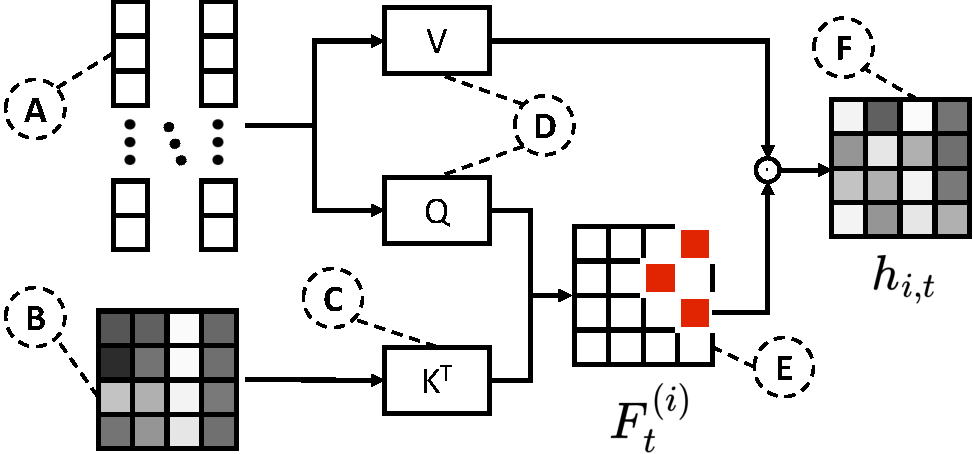
\includegraphics[width=0.75\columnwidth]{img/3-methodology/attention-diagram.pdf}
    \caption[Illustration of cross-attention mechanism]{Illustration of the cross-attention mechanism in an U-NET block: (A) the text embedding $X$; (B) the unconditioned hidden state $\hat{h}_{i,t}$;(C) the attention key $W_{k}^{(i)}\hat{h}_{i,t}$ ; (D) the attention query $W_{q}^{(i)}X$ and value $W_{v}^{(i)}X$ ; (E) the attention matrix $F_{t}^{(i)}$ (represented as red squares the activated attentions); (F) and the U-NET block output $h_{i,t}$ conditioned by the text embedding.}
    \label{fig:attention-diagram}
\end{figure}


When considering the denoising subnetwork $\epsilon_\theta$ within a Latent Diffusion Model (LDM), there are various architectural choices available. However, U-Nets \cite{UNET} have emerged as a popular option, due to their strong capabilities in image segmentation, and is the subnetwork used in Stable Diffusion (refer to Section \ref{sec:diffusion-models}). U-Nets consist of downsampling convolution blocks that preserve local context and upsampling deconvolutional blocks responsible for restoring the output to its original size \cite{DAAM}. This iterative transformation removes noise from a latent vector, ultimately producing an output image through the utilization of a Variational Autoencoder (VAE) \cite{rombach2022high}.


The denoising process operates in a lower-dimensional latent space, represented by 2D vectors denoted as $\ell_t\in \mathbb{R}^{w \times h}$ at a specific time-step $t$. In each iteration of this process, the U-NET's downsampling blocks generate a series of K intermediate states $\{ h_{i,t}^{\downarrow}\}_{i=1}^{K}$. These hidden states, with dimensions $\left \lceil \frac{w}{c^i} \right \rceil \times \left \lceil \frac{h}{c^i} \right \rceil$, gradually decrease in size as they pass through the downsampling blocks. The reduction factors $c^i$ are typically set to 1, 2, 4, and 8. Following the downsampling, the upsampling blocks scale up the downsampled hidden state $h_{K,t}^\downarrow$ to $\{ h_{i,t}^{\downarrow}\}_{i=1}^{K} \subset \mathbb{R}^{\left \lceil \frac{w}{c^i} \right \rceil \times \left \lceil \frac{h}{c^i} \right \rceil}$, effectively restoring the original dimension of the vector $\ell_t$ at the network's input. By iteratively applying this process, an approximation of the reverse diffusion process is achieved, enabling the reconstruction of an image from a noisy vector.

To incorporate textual information into the process, U-Net blocks from Stable Diffusion utilize multi-headed cross-attention layers that follow the attention mechanism proposed in the transformers architecture \cite{rombach2022high, vaswani2017attention}. This mechanism is illustrated in Figure \ref{fig:attention-diagram}. Specifically, in the case of a downsampling block, the U-Net takes a text embedding $X:= \left [ x_1; \cdots; x_{l_W}\right ] \in \mathbb{R}^{l_C \times l_W}$ consisting of $l_W$ tokens, along with the output of the fully convolutional layers of the block before conditioning, denoted as $\hat{h}_{i, t}^\downarrow$. The conditioned output $h_{i, t}^\downarrow$ of the block is then calculated as follows:


\begin{equation}
\label{eq:daam-multiscale}
\begin{gathered}
    h_{i,t}^{\downarrow} = F_t^{(i)} \left ( \hat{h}_{i, t}^{\downarrow}, X \right ) \cdot \left( W_v^{(i)\downarrow}  X \right), \\
     F_t^{(i)} \left ( \hat{h}_{i, t}^{\downarrow}, X \right ) = \text{softmax} \left( (W_q^{(i)\downarrow} \hat{h}_{i, t}^{\downarrow})  (W_k^{(i)\downarrow} X)^T / \sqrt{d} \right).
\end{gathered}
\end{equation}

In Equation \ref{eq:daam-multiscale}, the matrices $W_{k}^{(i)\downarrow}$, $W_{q}^{(i)\downarrow}$, and $W_{v}^{(i)\downarrow}$ are projection matrices with $l_{H}^{(i)}$ attention heads. These matrices transform the text embedding $X$ and $\hat{h}_{i, t}^{\downarrow}$ into vectors with dimensions $\left \lceil \frac{w}{c^i} \right \rceil \times \left \lceil \frac{h}{c^i} \right \rceil \times l_H^{(i)}$. Furthermore, the attention scores $F_{t}^{(i)\downarrow}$ have dimensions $\left \lceil \frac{w}{c^i} \right \rceil \times \left \lceil \frac{h}{c^i} \right \rceil \times l_H^{(i)} \times l_W$, which are obtained by concatenating the attention generated by each of the $l_W$ tokens.

To clarify the notation, we use $F_{t, k, h}^{(i)\downarrow}[x, y]$ to denote the attention array generated by the $k$-th token of the $h$-th multi-attention head in the $i$-th downsampling block at time $t \in \left [1, T \right]$. Similarly, in the case of upsampling blocks, we refer to their outputs as $h_{i, t}^\uparrow$ and their respective attention arrays as $F_{t, k, h}^{(i)\uparrow}[x, y]$. For brevity, when discussing an attention array that can be either from a downsampling or an upsampling block, we omit the arrow index $\downarrow$ or $\uparrow$.

In Equation \ref{eq:daam-multiscale}, it is important to note that the $\text{softmax}$ function is applied token-wise, independently for each attention head. Specifically, for each spatial coordinate $(x, y)$ and each head $h$, we have the following constraint:

\begin{equation}
    \label{eq:softmax-constraint}
    \sum_{k=1}^{l_W} F_{t, k, h}^{(i)}[x, y] = 1.
\end{equation}

This constraint ensures that, for each head and spatial point $(x, y)$, the attention is distributed among the different tokens.



To combine the attention arrays $F_{t, k, h}^{(i)} \in \mathbb{R}^{\left \lceil \frac{w}{c^i} \right \rceil \times \left \lceil \frac{h}{c^i} \right \rceil}$ from different blocks, interpolation is performed to unify them to the dimension of the original latent space $w \times h$. Due to the fully convolutional nature of the network, these arrays retain the same spatial distribution as the generated images. Therefore, scaling the attentions to different resolutions allows for their aggregation. We denote these scaled arrays as $\Tilde{F}_{t, k, h}^{(i)} \in \mathbb{R}^{w \times h}$. In the original formulation of DAAM \cite{DAAM}, the authors propose the use of bicubic interpolation for this scaling. However, in our preliminary experiments, we found that similar results in terms of IoU can be achieved using bilinear interpolation.


To create a heatmap from the scaled attention arrays, they are aggregated across all timesteps and heads using the following equation:

\begin{equation}
\label{eq:daam-summing}
    D_k^{\mathbb{R}}[x, y] := \sum_{t, i, l} \Tilde{F}_{t, k, l}^{(i) \downarrow}[x,y] + \Tilde{F}_{t, k, l}^{(i) \uparrow}[x,y].
\end{equation}

The resulting $D_k^{\mathbb{R}}$ represents a soft heat map, where higher values indicate a stronger attribution to the token $k$ (see Fig. \ref{fig:daam-example}). To convert this soft heat map into a binary mask, a threshold $\tau$ is applied relative to the maximum value of the attention map:

\begin{figure}
    \centering
    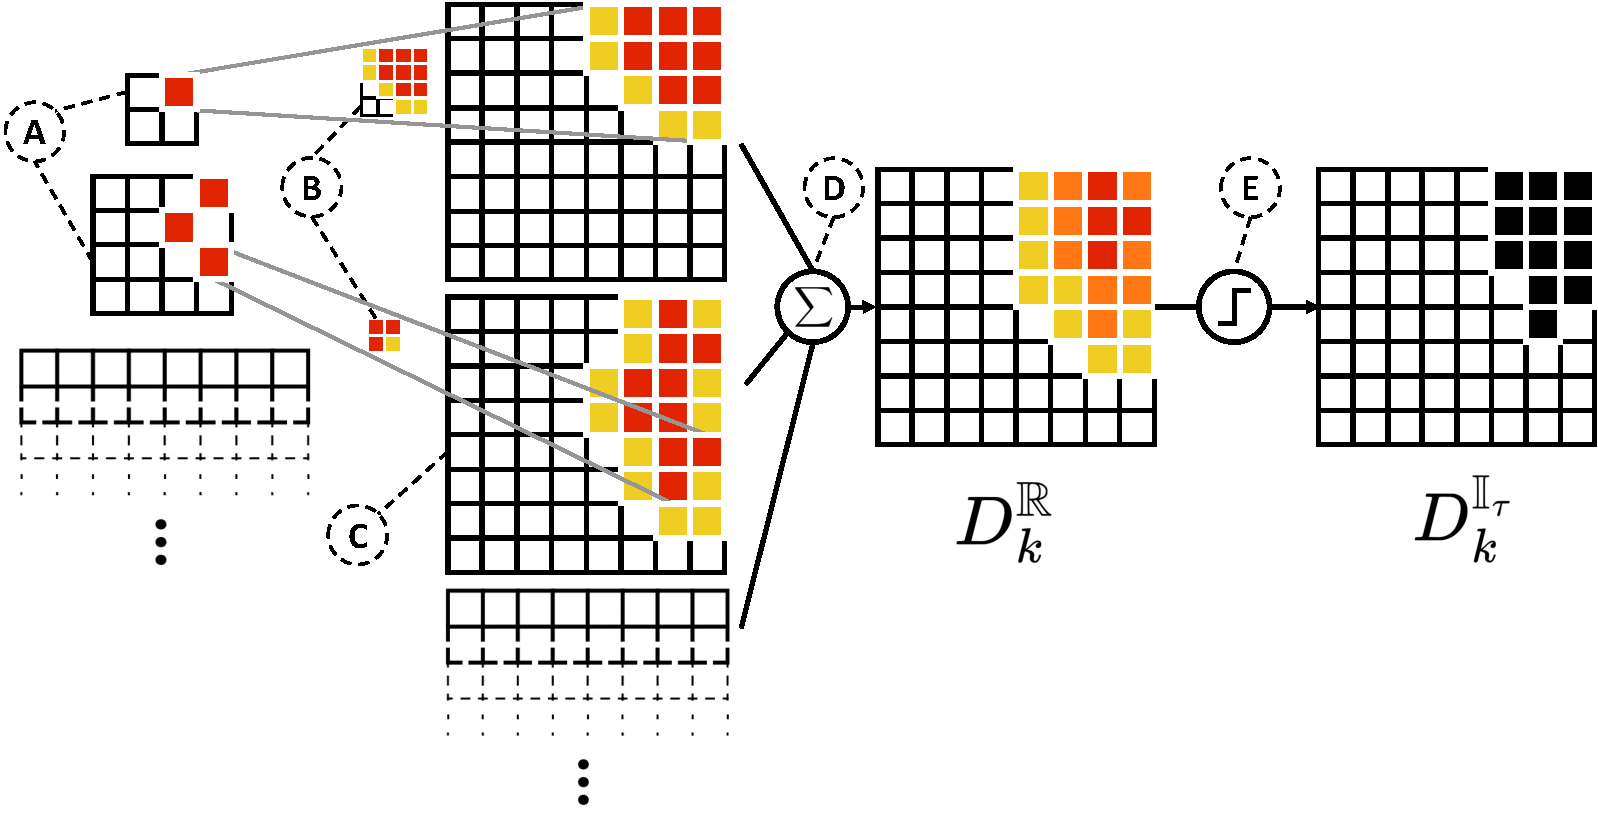
\includegraphics[width=1\columnwidth]{img/3-methodology/daam-diagram.pdf}
    \caption[Illustration of computing DAAM for some
word]{Illustration of computing DAAM for some
word: (A) the multiscale attention arrays from Eqn. \ref{eq:daam-multiscale}; (B) the bicubic interpolation  (C) resulting in expanded
maps; (D) summing the heatmaps across the layers,
as in Eqn. \ref{eq:daam-summing}; (E) and the thresholded maps. Source \cite{DAAM}.}
    \label{fig:daam}
\end{figure}


\begin{equation}
\label{eq:daam-binary}
    D_k^{\mathbb{I}_\tau}[x, y] := \mathbb{I}\left ( D_k^{\mathbb{R}}~\ge~\tau\cdot\max_{x, y}D_k^{\mathbb{R}} \right ).
\end{equation}

Here, $\mathbb{I}(\cdot)$ is the indicator function, and $\tau \in \left[0, 1 \right]$. The resulting binary mask highlights regions where the token $k$ is attributed. Figure \ref{fig:daam} provides an illustration of the DAAM construction process for a token.

DAAM serves as a powerful explainability technique for LDM, providing insights into how textual input information is synthesized and enabling the construction of semantic segmentation mechanisms. However, there are limitations to using these attention maps as ground truth for semantic segmentation tasks. For instance, binary masks depend on the threshold $\tau$, which requires further study to determine optimal values. Another limitation is that the original formulation of DAAM \cite{DAAM} does not consider generating heatmaps for tokens that are not present. This limitation prevents us from extracting masks for objects in the image, such as a tree in an urban environment, if it was not mentioned in the initial text.

Furthermore, we found that the influence area of a token does not always align with the annotation criteria of the desired semantic segmentation masks. This discrepancy arises from the semantic relationships learned by the network and the influence of the word on other parts of the scene.

These limitations make it challenging to use DAAM beyond its role as an explanation tool, especially for semantic segmentation tasks. In this work, we propose several modifications to extend the method and overcome these limitations in Sections \ref{cha:methodology-ov-daam} and \ref{cha:methodology-ov-daam-optimization}.


\section{Open Vocabulary-based DAAM}
\label{cha:methodology-ov-daam}

One of the main limitations of DAAM \cite{DAAM}, beyond its use as an explainability technique, is its restriction to generating attribution maps only for tokens present in the text prompt used to generate a sentence. This limitation becomes particularly significant when applying the method to generate semantic segmentation masks, as it would require all words to be present in the text that generated the image. In the example shown in Figure \ref{fig:daam-example}, where an image is generated with the prompt ``A car in an urban environment,'' it can be observed that besides the car, the urban scene also contains a sidewalk, a tree, and a building, for which the original method cannot generate attribution maps.

Although these tokens have not explicitly influenced the generation process, they are semantically related to elements in the generated scene. Hence, it raises the question of whether the attention they would have generated aligns with the regions corresponding to the respective objects in the image. The use of DAAM in semantic segmentation motivates the extension of the method in this regard. Furthermore, it allows for a deeper exploration of the model's internal workings, uncovering learned semantic relationships and biases.

In this section, we propose two modifications to the original formulation of 
DAAM \cite{DAAM}, which expand its capabilities by incorporating attention maps for out-of-vocabulary tokens.

First, we introduce the ``Open Vocabulary DAAM'' modification. In this approach, the original DAAM process is divided into two steps: generating the image and capturing the hidden states, followed by generating the attention matrices using an arbitrary text embedding. This modification enables the generation of heatmaps for arbitrary prompts and their tokens. However, it is important to note that the attention captured by each token is relative to the attention captured by other tokens due to the token-wise softmax operation. One limitation of this first approach is that to generate an attention heatmap for a specific word, it will be necessary to include it in a context sentence with other tokens that capture the attention of the non-interested regions.

Furthermore, we present the ``Linear Open Vocabulary DAAM'' modification. In this variant, we remove the softmax operation and directly aggregate the attention linear projections. This modification aims to explore the impact of removing the softmax operation on attention patterns and the resulting heatmaps.

We describe the procedures for generating attention maps from arbitrary sentences, addressing the challenges associated with tokens not present in the prompt.

\subsection{Open Vocabulary DAAM}
\label{sec:methodology-ov-daam-softmax}


In this subsection, we propose a modification to the construction of DAAM\cite{DAAM} to enable the evaluation of attention heatmaps for text prompts different from those used to generate the image, which guided the reverse diffusion process. To achieve this, we introduce a two-phase approach for constructing the attention maps.

In the first phase, referred to as the ``collection'' phase, a text prompt $X := [x_1; \cdots; x_{l_W}]$, referred to as the generator text embedding, is provided. An image is generated using the LDM, and during this process, the outputs of the downsampling and upsampling blocks of the U-NET prior to conditioning are saved. These outputs, denoted as $\{\hat{h}_{i,t}^{\downarrow}\}_{i=1}^{K}$ and $\{\hat{h}_{i,t}^{\uparrow}\}_{i=1}^{K}$ in equation \ref{eq:daam-multiscale}, contain spatial information about the generated image. In the original DAAM formulation \cite{DAAM}, these hidden states are used as input to the cross-attention layers of the U-NET, which incorporate the textual information and generate the attention arrays $F_{t}^{(i)}$ for constructing the DAAMs.

In the second phase, utilizing the collected hidden states $\hat{h}_{i,t}$, we construct the attention arrays based on a new text prompt. This text prompt can have different lengths and contain different tokens. Given the new text embedding $X':= [x_1; \cdots; x_{l_{W'}}] \in \mathbb{R}^{l_C \times l_{W^\prime}}$, referred to as the contextual text embedding, we generate the attribution arrays as follows:

\begin{equation}
\label{eq:daam-multiscale-ov}
\begin{gathered}
     F_{X,t}^{(i)} \left (X^\prime \right ) = \text{softmax} \left( (W_q^{(i)\downarrow} \hat{h}_{i, t}^{\downarrow})  (W_k^{(i)\downarrow} X^\prime )^T / \sqrt{d} \right).
\end{gathered}
\end{equation}

Here, $\hat{h}_{i, t}^{\downarrow}$ represents the unconditioned hidden states collected during the previous step. This computation of the attention arrays is essentially the same as the one used in the original formulation of DAAM \cite{DAAM}, utilizing the hidden states from the generator text embedding and the contextual embedding as keys in the cross-attention.
The notation $F_{X,t}^{(i)}$ is used to refer to this attention array, indicating that the hidden states $\hat{h}_{i,t}$ were generated using the text embedding $X$. Similar to Equation \ref{eq:daam-multiscale}, the $\text{softmax}$ function is applied token-wise, independently for each attention head (see the constraint in Equation \ref{eq:softmax-constraint}).

Once the new attention arrays are constructed, we can obtain the DAAMs for the text prompt $X'$ following the same methodology as in the original method \cite{DAAM}. Firstly, we rescale the spatial dimensions of the attention arrays, denoted as $\tilde{F}_{X,t}^{(i)}$, to have dimensions $w \times h \times l_{H}^{(i)} \times l_{W^\prime}$.

After constructing the rescaled attention arrays, we can generate the new heatmap based on attention by aggregating the heads from all blocks and timesteps of the process. Specifically, we have:

\begin{equation}
\label{eq:daam-summing-ov}
    D_{X,k}^{\mathbb{R}}[x, y] \left ( X^\prime \right ) := \sum_{t, i, l} \Tilde{F}_{X, t, k, l}^{(i) \downarrow}[x,y]\left ( X^\prime \right ) + \Tilde{F}_{X, t, k, l}^{(i) \uparrow}[x,y]\left ( X^\prime \right ).
\end{equation}


The entire process is illustrated in Figure \ref{fig:daam-ov-diagram}. Similar to the original version of DAAM, these modifications allow for the generation of attention heatmaps for arbitrary text prompts, providing insights into the attention patterns in the image.

  \begin{figure}
    \centering
    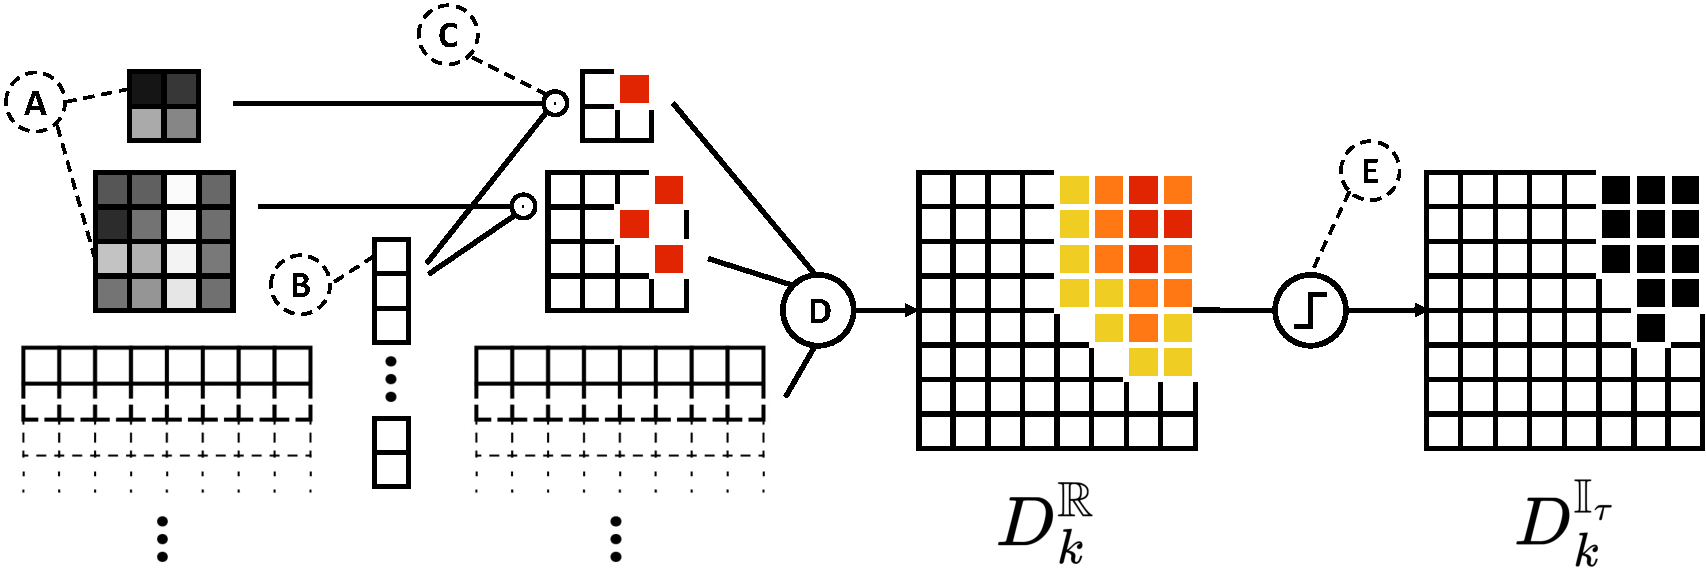
\includegraphics[width=1\columnwidth]{img/3-methodology/diagram-ov-daam.pdf}
    \caption[Illustration of computing DAAM for open
vocabulary]{Illustration of computing DAAM for open vocabulary: the hidden states $W_{q}^{(i)}\hat{h}_{i,t}^{\downarrow}$ stored during the reverse diffusion process (A); the text embedding (B); the cross-attention matrices (C) used to compute the DAAM (D); and the thresholded maps (E). Modification of figure from \cite{DAAM}.}
    \label{fig:daam-ov-diagram}
\end{figure}


Figure \ref{fig:daam-ov-example-softmax} illustrates the results of generating attention maps on the image with the prompt ``a car in an urban environment'' (see Figure \ref{fig:daam-example-image}) for the tokens ``tree,'' ``building,'' and ``sidewalk.'' As a context phrase $X'$ for extracting the attention, the phrase ``a car and a \textlangle token\textrangle\ in an urban environment'' has been used, where \textlangle token\textrangle\ represents each of the three words depicted in Figures \ref{fig:daam-ov-example-image} to \ref{fig:daam-ov-example-image-2}. The figure shows that despite not being present in the generator text prompt, the tokens are indeed related to semantically relevant areas. The attribution of the ``tree'' token is primarily focused on the tree's leaves, ``building'' is attributed to the buildings in the background, and ``sidewalk'' is attributed to the ground in the image. Therefore, it appears that the attention information successfully extends to tokens that were not present during the generation process.



\begin{figure}
\centering
  % First column
  \begin{subfigure}{0.30\columnwidth}
   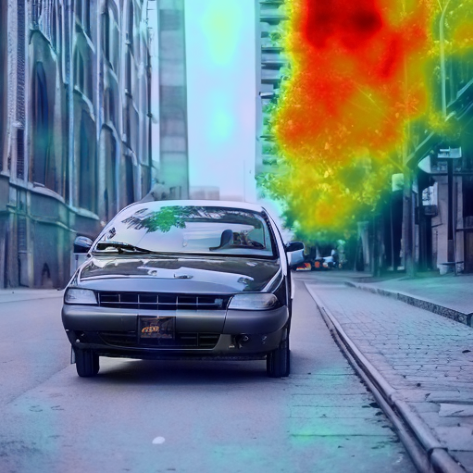
\includegraphics[width=\columnwidth]{img/3-methodology/example_ov_daam_heatmap_tree_without_special_tokens.png}
   \caption{``tree''}
   \label{fig:daam-ov-example-image}
  \end{subfigure}
  \begin{subfigure}{0.30\columnwidth}
   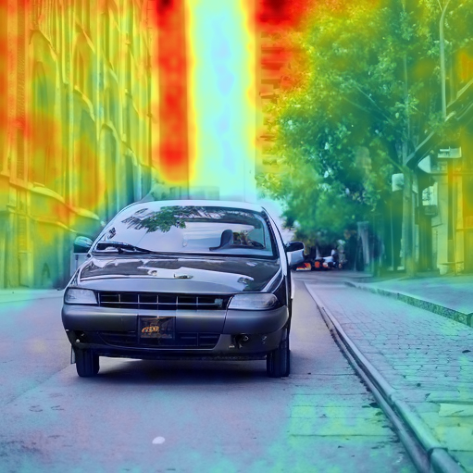
\includegraphics[width=\columnwidth]{img/3-methodology/example_ov_daam_heatmap_building_without_special_tokens.png}
   \caption{``building''}
   \label{fig:daam-ov-example-image-1}
  \end{subfigure}
  \begin{subfigure}{0.30\columnwidth}
   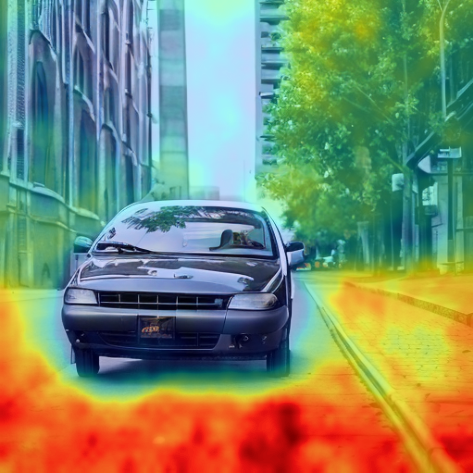
\includegraphics[width=\columnwidth]{img/3-methodology/example_ov_daam_heatmap_sidewalk_without_special_tokens.png}
   \caption{``sidewalk''}
   \label{fig:daam-ov-example-image-2}
  \end{subfigure}
  \caption[Example of Open Vocabulary DAAMs]{Example of Open Vocabulary DAAMs: An image generated with the prompt ``A car in an urban environment'' with overlaid attention maps for the tokens ``tree'' (\ref{fig:daam-ov-example-image}), ``building'' (\ref{fig:daam-ov-example-image-1}), and ``sidewalk'' (\ref{fig:daam-ov-example-image-2}). The attention maps were extracted using the contextual prompt ``A car and a \textlangle token\textrangle\ in an urban environment,'' where \textlangle token\textrangle\ represents each of the depicted words.}
  \label{fig:daam-ov-example-softmax}
  \end{figure}


This modification has significant potential as it effectively extends the attribution of different words in an image generated by an LDM to any arbitrary text prompt. However, since the attention is relative to the other tokens in the context phrase, studying the attribution of a single token becomes complex. This limitation arises when generating segmentation masks for objects in the scene. Nonetheless, it can still be valuable for other applications, such as understanding how modifications to a prompt influence image generation, enabling the construction of better prompts for LDMs.

\subsection{Linear Open Vocabulary DAAM}
\label{sec:methodology-ov-daam-linear}


One of the main limitations of the first proposed modification, the ``Open Vocabulary DAAM,'' is the requirement of defining a context phrase to extract attention maps for tokens that are not present in the prompt used to generate the image. For example, in Figure \ref{fig:daam-ov-example-softmax}, attention masks for ``tree,'' ``building,'' and ``sidewalk'' were generated using the context phrase ``A car and a \textlangle token\textrangle\ in an urban environment''. This dependence on a context phrase makes it challenging to use this extension as an explainability method for understanding the relation of standalone words in the image, as well as for generating attention masks for individual objects in synthetic images. The attribution generated by this method strongly relies on how the contextual phrase is constructed. Thus, there is a need to find a way to extract attention without considering the attention of other tokens.

After conducting several preliminary experiments to study the role of the softmax function in the attribution of different tokens in the phrase, it was found that aggregating the attentions of a single token without applying $\text{softmax}$ still resulted in attention heatmaps focused on the same areas as when using a tailored context phrase. Therefore, the second proposed variation, called ``Linear Open Vocabulary DAAM,'' is a modification of the previous method without the application of $\text{softmax}$.


To generate a Linear DAAM, the first step is to perform a collection phase. This is done by generating an image with a text prompt $X$ and capturing the hidden states $\hat{h}_{i,t}$. This collection phase is identical to the one proposed in the previous extension (see section \ref{sec:methodology-ov-daam-softmax}).


Once the hidden states have been captured, we proceed to compute the attention of an individual token without applying the softmax function, as defined in Equation \ref{eq:daam-multiscale-ov}. Specifically, for a given token embedding $x$ for which we aim to generate an attribution map, the attention is calculated as:

\begin{equation}
\label{eq:daam-multiscale-ov-linear}
\begin{gathered}
     L_{X,t}^{(i)} \left (x \right ) = (W_q^{(i)\downarrow} \hat{h}_{i, t}^{\downarrow})  (W_k^{(i)\downarrow} x )^T \, .
\end{gathered}
\end{equation}

In this context, the attention array $L_{X,t}^{(i)}\in \mathbb{R}^{\left \lceil \frac{w}{c^i} \right \rceil \times \left \lceil \frac{h}{c^i} \right \rceil \times l_{H}^{(i)}}$ corresponds to the result of computing the dot product between the query projection $W_q^{(i)\downarrow} \hat{h}_{i, t}^{\downarrow}$ and the key projection $W_k^{(i)\downarrow} x$. This computation enables us to capture the token's relevance within the image, without the incorporation of the softmax normalization utilized in Equation \ref{eq:daam-multiscale-ov}.
Subsequently, the attention arrays are rescaled to dimensions $w \times h \times l_{H}^{(i)}$, denoted as $\tilde{L}_{X,t}^{(i)}$, to facilitate their aggregation. Finally, all the attention arrays are combined into a unified heatmap by summing them together.

\begin{equation}
\label{eq:daam-summing-ov-linear}
    {LD}_{X}^{\mathbb{R}}[x, y] := \sum_{t, i, l} \Tilde{L}_{X, t, l}^{(i) \downarrow}[x,y] + \Tilde{L}_{X, t, l}^{(i) \uparrow}[x,y].
\end{equation}


\begin{figure}
\centering
  % Second column
  \begin{subfigure}{0.30\columnwidth}
   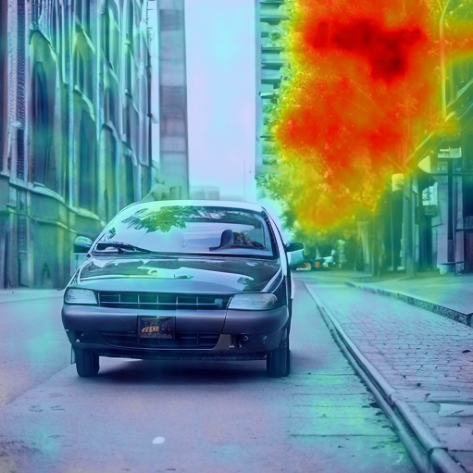
\includegraphics[width=\columnwidth]{img/3-methodology/example_ov_daam_heatmap_tree_without_context.png}
   \caption{``tree''}
   \label{fig:daam-ov-example-image-3}
  \end{subfigure}
  \begin{subfigure}{0.30\columnwidth}
   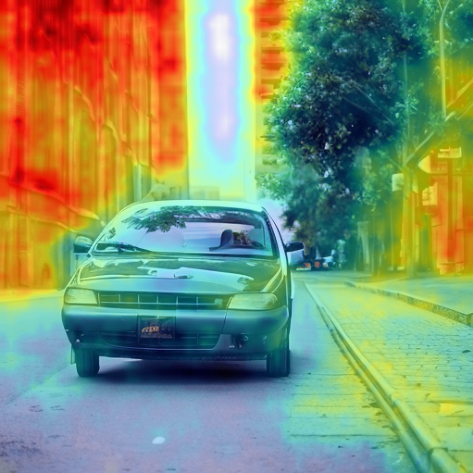
\includegraphics[width=\columnwidth]{img/3-methodology/example_ov_daam_heatmap_building_without_context.png}
   \caption{``building''}
   \label{fig:daam-ov-example-image-4}
  \end{subfigure}
  \begin{subfigure}{0.30\columnwidth}
   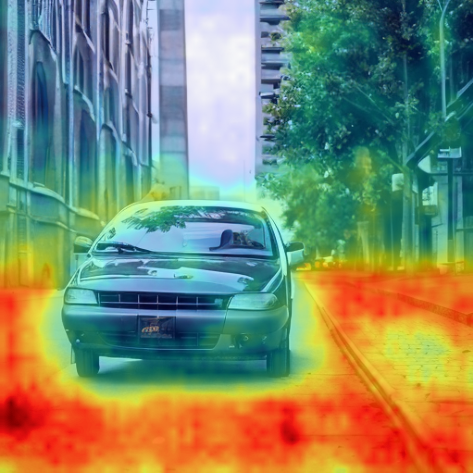
\includegraphics[width=\columnwidth]{img/3-methodology/example_ov_daam_heatmap_sidewalk_without_context.png}
   \caption{``sidewalk''}
   \label{fig:daam-ov-example-image-5}
  \end{subfigure}
  \caption[Example of Linear Open Vocabulary DAAMs]{Example of Linear Open Vocabulary DAAMs: An image generated
with the prompt ``A car in an urban environment'' with overlaid linear attention maps for the
tokens ``tree'' (\ref{fig:daam-ov-example-image-3}), ``building'' (\ref{fig:daam-ov-example-image-4}), and ``sidewalk'' (\ref{fig:daam-ov-example-image-5}).}
  \label{fig:daam-ov-example-linear}
  \end{figure}

In Figure \ref{fig:daam-ov-example-linear}, the results of three linear attention maps, denoted as ${LD}_{X}^{\mathbb{R}}$ in eq. \ref{eq:daam-summing-ov-linear}, are presented for the tokens ``tree,'' ``building,'' and ``sidewalk'' on the example image generated with the text prompt ``A car in an urban environment.'' The example demonstrates how these heatmaps generate attention in the same regions as their $\text{softmax}$ counterparts, without the need for a context phrase that interferes with their attention. This characteristic enhances their utility as an explainability method, simplifying the examination of biases acquired by a model or the generation of semantic segmentation masks based on a single word.

However, despite the potential of this method as an explainability technique for LDMs, it is still limited as a standalone approach for extracting ground truth in semantic segmentation tasks. A key limitation shared with the original DAAM approach \cite{DAAM} is that the regions attributed to a word may not align with the semantic segmentation mask assigned to the class represented by that word. For instance, in Figure \ref{fig:daam-ov-example-image-5}, it is evident that the attribution of the word ``sidewalk'' also extends attention to the road section, which is typically labeled as a distinct class in urban scene segmentation tasks. In other cases, the word may generate attention in other areas due to different learned semantic relationships within the network. To rigorously investigate this issue, an optimization approach for searching the text embedding that maximizes the Intersection over Union (IoU) with the target region is proposed in Section \ref{cha:methodology-ov-daam-optimization}.


\section{Prompt optimization via DAAM}
\label{cha:methodology-ov-daam-optimization}


The proposed extensions of DAAM for open vocabulary usage provide increased flexibility as an explainability tool. They allow us to highlight the semantic relationships learned by a Latent Diffusion Model (LDM), such as Stable Diffusion, by examining the influence of words on its internal attentions. However, initial tests showed that the attribution maps extracted for object nouns in generated images often do not align with the corresponding ground truth semantic segmentation masks. Although these maps demonstrate semantic coherence, they also include unwanted regions, which presents challenges for their application beyond explainability.

For instance, the attribution map for the word ``building'' (Figure \ref{fig:daam-ov-example-image-4}) extended its influence to the sidewalk, likely due to their semantic association within the urban context. In another case (Figure \ref{fig:daam-ov-example-image-5}), the ``sidewalk'' map also encompassed the road area, deviating from the desired segmentation. Such irregularities impede the effective use of attention maps in semantic segmentation tasks.

To address these limitations, we propose approaching the problem as a minimization problem solved through gradient descent on the extension of DAAM for Open Vocabulary proposed in this work (Fig. \ref{fig:daam-optimization-diagram} illustrates this process). We will focus on formulating the method in its simplest variant: the search for a single token, $x$, that maximizes a specific region based on its Linear DAAM.


\begin{figure}
    \centering
    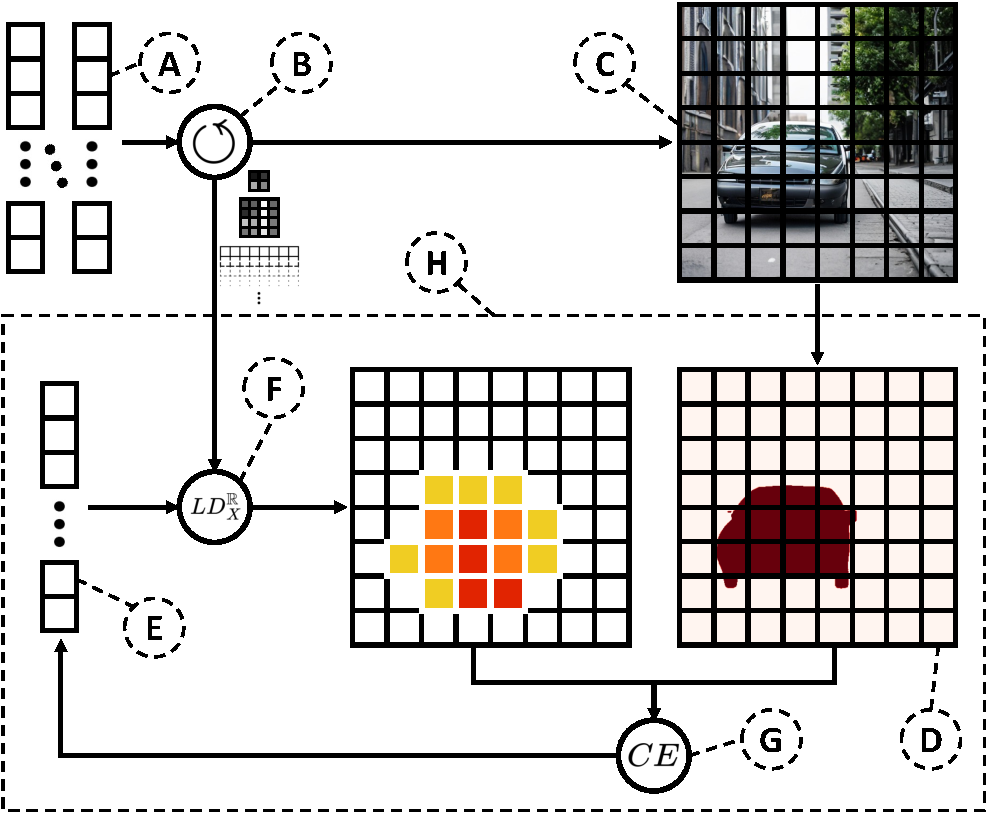
\includegraphics[width=0.8\columnwidth]{img/3-methodology/optimization-diagram.pdf}
    \caption[Prompt Optimization Process Diagram]{Prompt Optimization Process Diagram. The diagram illustrates the following steps: (A) Input of a text embedding $X$ into a LDM (B), resulting in the generation of a synthetic image (C). (D) The target mask is annotated. A token embedding $x$ (E) is utilized to generate the Open Vocabulary DAAM (F). The error between the target mask and the attention heatmap is calculated, and gradients are backpropagated (G) and $x$ is updated. (H) This process is repeated within an optimization loop.}
    \label{fig:daam-optimization-diagram}
\end{figure}

A Linear DAAM, denoted as ${LD}^\mathbb{R}_X$, can be understood as a function that takes a token embedding, $x\in \mathbb{R}^{l_C}$ and a set of hidden states, ${LD}^\mathbb{R} ( X^\prime; \hat{h}_{1, 1}^\downarrow, \cdots, \hat{h}_{T, K}^\uparrow )$, and generates an attention map. In this optimization, we keep the hidden states fixed and consider the DAAM solely as a function of $x$, indicated by the subscript $X$ to represent the text embedding that generated these states. In other words, ${LD}^\mathbb{R}_X\left ( \cdot \right):\mathbb{R}^{l_C} \to \mathbb{R}^{w \times h}$. To formulate the optimization problem, we introduce a binary mask, $G_X \in \mathbb{R}^{w \times h}$, representing the ground truth of the target influential area. Our objective is to minimize a cost function $C$, which should be differentiable, in charge of measure the divergence between the output of the Linear DAAM and the ground truth $G_X$:

\begin{equation}
\label{eq:objective-optimization}
    \hat{x} = \arg\min_{x} C \left ( {LD}_X^{\mathbb{R}}\left ( x \right ), G_X \right ) .
\end{equation}

This objective function (Eq. \ref{eq:objective-optimization}) is differentiable with respect to $x$, as ${LD}_X^{\mathbb{R}}$ is the sum of linear projections of the input token (Eq. \ref{eq:daam-multiscale-ov-linear}) and spatial interpolations of these projections (Eq. \ref{eq:daam-summing-ov-linear}). Therefore, we can optimize the objective function using gradient descent. Figure \ref{fig:daam-optimization-diagram} illustrates this iterative optimization process, where the token embedding is updated based on the gradients of the objective function.

We found that the cross-entropy loss between the soft heatmap and the ground truth worked effectively for the optimization. The cross-entropy loss is defined as:

% Nota para Roberto sobre notacion: 
% Se que la letra "x" se utiliza tanto para indicar el token siendo maximizado
% como la coordenada espacial x (de las x,y). Es notación heredada del paper
% de DAAM, la utilizan de forma repetida. La habría cambiado en esta memoria,
% pero es que no me quedan letras y no me apetece 
% meter letras griegas y cambiar la notacion del paper original XD
% Pasa lo mismo con la letra h, que se usa para la dimension w x h
% y como variable en los sumatorios que indica suma sobre multihead attentions.

\begin{equation}
\label{eq:cross-entropy}
    CE_{loss} \left ({LD}_X^{\mathbb{R}}, G_X \right ) = - \sum_{x, y} G_X [x, y]\cdot \log \left ( {LD}^{\mathbb{R}}_X [x, y] \right ) .
\end{equation}

To compute the cross-entropy loss, the heatmap needs to be normalized in the range of $[0, 1]$. Since the linear DAAM is a sum of linear projections and is not inherently normalized like softmax-based heatmaps. We employed a linear scaling, also known as min-max scaling, to resize the heatmap values to the desired range of $[0, 1]$. This normalization effectively scaled the heatmap values, ensuring consistent visualization of the heatmaps throughout the optimization process. For clarity, the normalization step has not been included in the notation of Equation \ref{eq:cross-entropy}.

\begin{figure}
\centering
  \begin{subfigure}{0.30\columnwidth}
   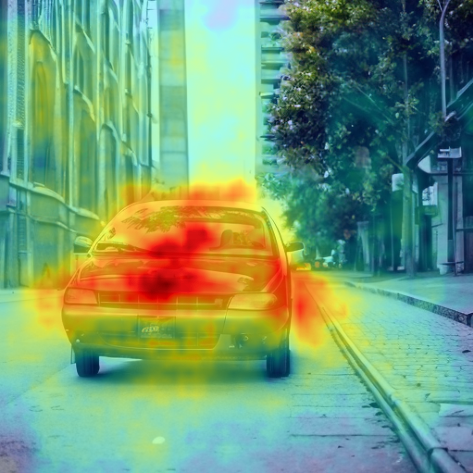
\includegraphics[width=\columnwidth]{img/3-methodology/initial_mask.png}
   \caption{Initial heatmap}
   \label{fig:optimization-initial-mask}
  \end{subfigure}
  \begin{subfigure}{0.30\columnwidth}
   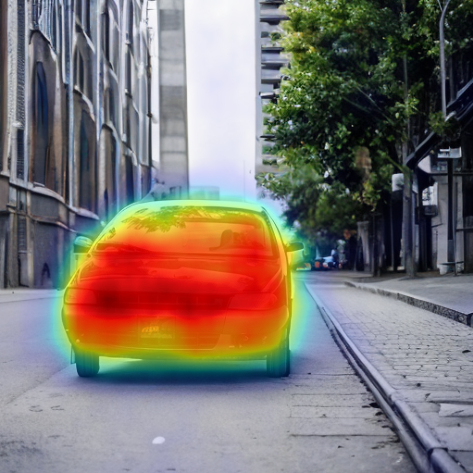
\includegraphics[width=\columnwidth]{img/3-methodology/optimized_mask.png}
   \caption{Optimized heatmap}
   \label{fig:optimization-optimized-mask}
  \end{subfigure}
  \begin{subfigure}{0.30\columnwidth}
   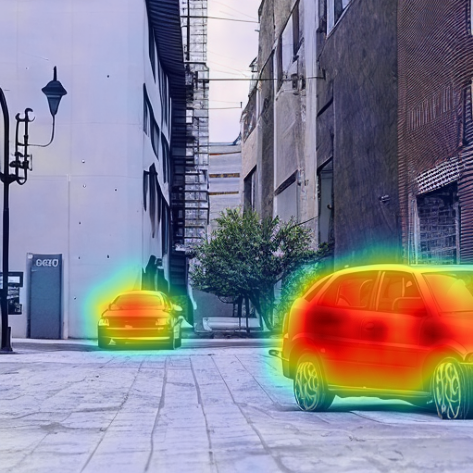
\includegraphics[width=\columnwidth]{img/3-methodology/extrapolated_mask.png}
   \caption{Transferred heatmap}
   \label{fig:optimization-extrapolated-mask}
  \end{subfigure}
  \caption[Example of Optimization via DAAM]{Example of Optimization via DAAM. The figure showcases the optimization process applied to the example image (Fig \ref{fig:daam-example-image}). It includes the initial Linear DAAM of the token ``car'' overlaid on the image (Fig. \ref{fig:optimization-initial-mask}), the optimized heatmap generated by $\hat{x}$ (Fig. \ref{fig:optimization-optimized-mask}), and the Linear DAAM of $\hat{x}$ on a different image (Fig. \ref{fig:optimization-extrapolated-mask}).}
  \label{fig:example-optimization}
  \end{figure}


Figure \ref{fig:example-optimization} visually presents the optimization results conducted on the example image discussed throughout this chapter (Fig. \ref{fig:daam-example-image}). 
In Fig. \ref{fig:optimization-initial-mask}, we observe the Linear DAAM generated for the token ``car.'' A comparison with the DAAM generated using the original non-linear method (Fig. \ref{fig:daam-example-image-3}) reveals notable differences in behavior. While the resulting mask maintains its focus on the car, it exhibits a broader influence that extends beyond the immediate region. This is because the absence of softmax normalization between tokens in a text embedding allows the attention to encompass surrounding background areas.

To tackle this issue, we utilize ``car'' as the initial token $x$ for the optimization process. The resulting heatmap generated by $\hat{x}$ after optimization is depicted in Figure \ref{fig:optimization-optimized-mask}. It can be observed that the resulting area more precisely delineates the region surrounding the car, without attracting attention from the urban environment.

To assess the semantic information encapsulated within $\hat{x}$ and its generalizability, we evaluate its performance on a different image generated by the LDM. As shown in Figure \ref{fig:optimization-extrapolated-mask}, we observe a scene featuring two cars on a street. Notably, the optimized vector effectively generates attention around both car instances, indicating the transferability of learned semantic knowledge to influence attentions in diverse image contexts.

Furthermore, this approach is also valid for optimizing Open Vocabulary DAAMs, in which we would need to jointly optimize a text embedding $X^\prime = [x_1, ...; x_{l_{W^\prime}}]$ with a segmentation mask for each token in the phrase. In this case $D^\mathbb{R}_X\left ( \cdot \right):\mathbb{R}^{l_C \times l_{W^\prime}} \to \mathbb{R}^{w \times h \times l_{W^\prime}}$. 

In the general case, where $X^\prime$ is optimized across multiple images generated with text prompts $\{X_j\}_{j=1}^N$, where the length of the tokens $X_j$ can vary, the objective function is defined as follows:

\begin{equation}
\label{eq:general-objective}
    \hat{X^\prime} = \arg\min_{X^\prime} \sum_{j=1}^N \sum_{k=1}^{l_{W^\prime}} C \left ( D_{ X_j, k}^{\mathbb{R}}\left ( X^\prime \right ), G_{X_j, k} \right ) .
\end{equation}

Where for practical experiments we use as loss $C$ the cross entropy $CE_{loss}$.
This objective function (Eq. \ref{eq:general-objective}) shares similarities with the loss function employed in training a semantic segmentation model. However, unlike traditional training with images, we utilize the attentions generated during their generation in the LDM (indexed by $j$). Instead of working with multiple semantic classes as the output objective, we focus on optimizing the activations of multiple tokens (indexed by $k$). Moreover, instead of updating the weights of the model, our optimization process revolves around refining the input text embedding ($X^\prime \in \mathbb{R}^{l_C \times l_{W^\prime}}$) . It is important to emphasize that, similar to a semantic segmentation model, we utilize binary masks as ground truth for each image and class/token in the training dataset ($G_{X_j}, k$). Figure \ref{fig:daam-general-optimization-diagram} illustrates the procedure proposed to optimize this function.
%Experiments conducted (Sec. \ref{sec:experiment-optimization}) indicate that only 1 or 2 annotated images for class are sufficient to optimize the text embedding for a simple dataset.

In the following chapter, we conduct practical experiments aimed at analyzing the potential of prompt optimization via DAAM method in generating accurate segmentation masks. These experiments explore the effectiveness of the optimization process by assessing the quality and alignment of the generated masks in comparison to the ground truth annotations. Moreover, we investigate the generalization capabilities of the optimized text embeddings across a diverse range of images generated by the LDM.

\begin{figure}
    \centering
    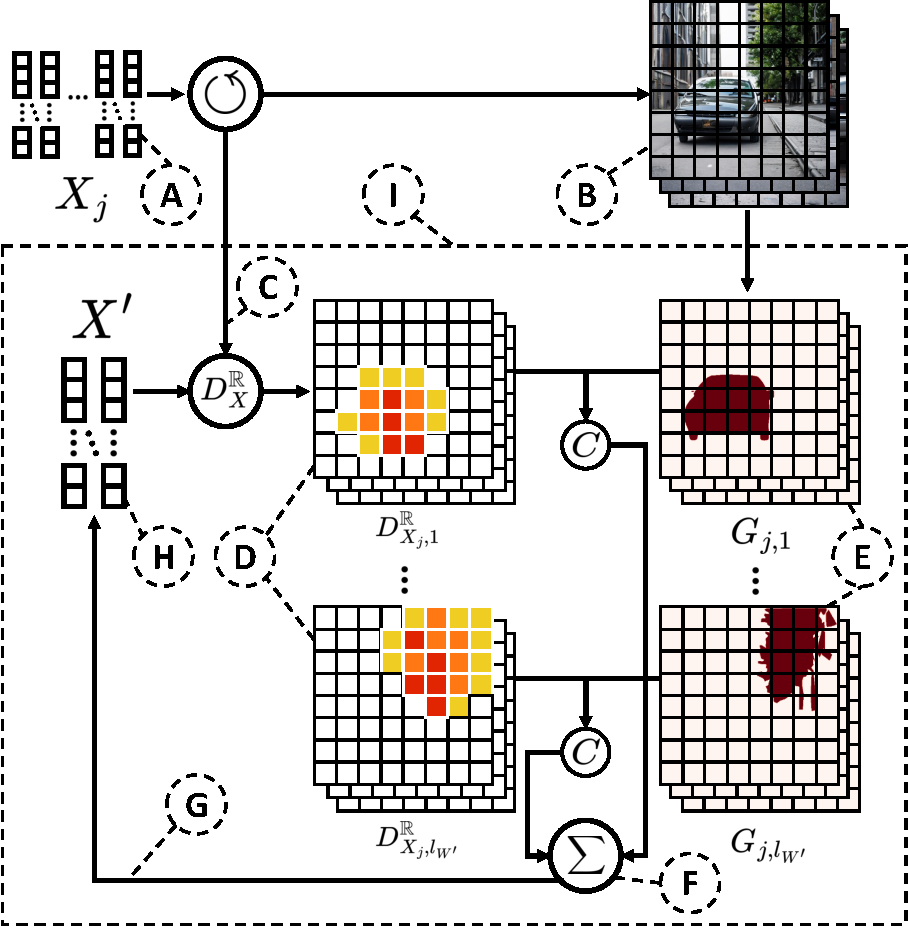
\includegraphics[width=0.8\columnwidth]{img/3-methodology/general-optimization.pdf}
    \caption[Prompt Optimization Diagram. General case.]{Optimization process of DAAM in the general case. The diagram illustrates the following steps: (A) Inputting the set of text embeddings $X_j$ into a LDM, resulting in the generation of synthetic images (B). The attentions generated by the LDM are fixed in the DAAM function (C). DAAM generates heatmaps (D) corresponding to the target masks (E), which are used to compute the loss for each image and token (F). The gradients of the loss are propagated (G) and employed to update the text embedding $X^\prime$ (H). This iterative process occurs within an optimization loop (I).}
    \label{fig:daam-general-optimization-diagram}
\end{figure}
